\subsection*{Problema 09}

\noindent\textbf{Enunciado:} Calcular la integral:
\begin{equation*}
\int \dfrac{x^4 - 6x^3 + 12x^2 + 6}{x^3 - 6x^2 + 12x - 8} \, dx
\end{equation*}

\noindent\textbf{Solución:} Primero, observamos que el denominador es el binomio al cubo expandido:
\begin{equation*}
x^3 - 6x^2 + 12x - 8 = (x - 2)^3
\end{equation*}

Dado que el grado del numerador es mayor que el del denominador, realizamos la división polinómica de $x^4 - 6x^3 + 12x^2 + 6$ entre $x^3 - 6x^2 + 12x - 8$. Al dividir, obtenemos un cociente de $x$ y un residuo de $6$. Es decir:
\begin{equation*}
\dfrac{x^4 - 6x^3 + 12x^2 + 6}{(x - 2)^3} = x + \dfrac{6}{(x - 2)^3}
\end{equation*}

Reescribimos la integral original utilizando esta descomposición:
\begin{equation*}
\int \left( x + \dfrac{6}{(x - 2)^3} \right) dx
\end{equation*}

Separamos la integral en dos términos más sencillos:
\begin{equation*}
= \int x \, dx + \int \dfrac{6}{(x - 2)^3} \, dx
\end{equation*}

La primera integral es inmediata:
\begin{equation*}
\int x \, dx = \dfrac{x^2}{2}
\end{equation*}

Para la segunda integral, aplicamos sustitución simple haciendo $u = x - 2$, de modo que $du = dx$:
\begin{align*}
\int \dfrac{6}{(x - 2)^3} \, dx &= 6 \int u^{-3} \, du \\
&= 6 \left( \dfrac{u^{-2}}{-2} \right) \\
&= -\dfrac{3}{u^2}
\end{align*}

Regresando a la variable original $x$:
\begin{equation*}
-\dfrac{3}{u^2} = -\dfrac{3}{(x - 2)^2}
\end{equation*}

Finalmente, combinamos ambos resultados y añadimos la constante de integración $C$:
\begin{equation*}
\dfrac{x^2}{2} - \dfrac{3}{(x - 2)^2} + C
\end{equation*}

\begin{figure}[H]
	\centering
	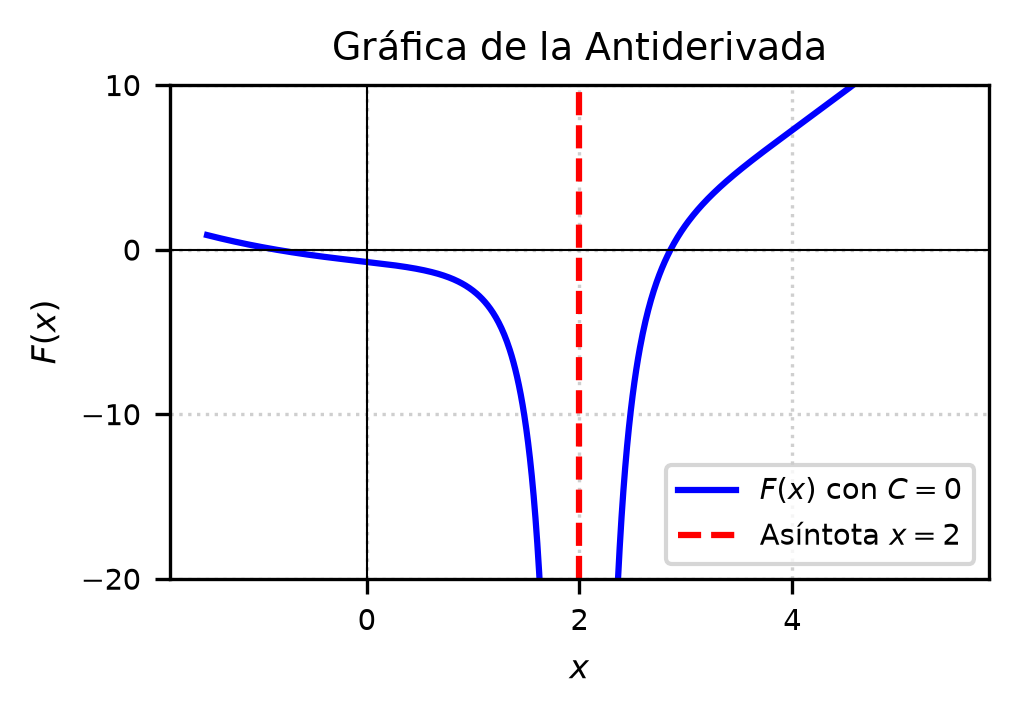
\includegraphics[width=\columnwidth]{semana_03/graficas/SEM03_P09_grafica.png}
	\caption{Representación gráfica de $f(x)$ y su antiderivada $F(x)$ evaluada para la constante de integración $C = 0$ (Problema 09).}
	\label{fig:problema09}
\end{figure}
